\paragraph{}
Dans cette partie nous allons présenter plus en détails l'architecture globale du projet d'application mobile de Neuflize OBC. Comme nous l'avons vu précédemment, ce projet est basé sur une architecture multicouches dont la structure est représentée dans sa globalité en annexe \ref{a2}. Nous allons maintenant décrire chacune des couches afin de comprendre le fonctionnement du projet. Cependant, les technologies employées étant nombreuses, il serait peu pertinent de toutes les expliciter, ainsi seul l'essentiel en lien avec le stage sera ici décrit. Toutefois, il est possible de retrouver une explication des différentes briques en annexe.

\subsection{Axway API Gateway}
\label{axway}

	Deux instances de l'API Gateway d'Axway ont été installées en mode « actif/actif » afin d'assurer la mise en place de la couche \textit{security} et celle de la couche \textit{management}. La répartition de charge est gérée par l'instance positionnée en amont. \\
		
	L'API Gateway de la couche security est le serveur traitant les appels API. Cette dernière est en charge de la sécurité applicative des appels vers la couche API Management. Elle est positionnée dans le tiers 1, reçois les appels « HTTPS » et a principalement pour objectif d’effectuer les actions suivantes : \\
	
	\begin{itemize}
		\item Vérifier la validité des certificats partenaires
		\item Filtrer les requêtes entrantes 
		\item Agir comme un pare-feu applicatif afin de vérifier le contenu des messages REST
		\item Répartir la charge vers les composants en aval
		\item Protéger le SI en limitant le nombre d’appels API via un mécanisme de régulation du traffic et en limitant le nombre d'appels au SI via un mécanisme de cache
		\item Collecter et tracer les exécutions pour la SLA (Service Level Agreement) \\
	\end{itemize}
	
	La couche API management, dans le tiers 2, permet de configurer et d’exposer les API. Elle contient également un mini serveur http afin de proposer des pages statiques d’authentification utilisateur. Elle assure les fonctionnalités suivantes : \\
	
	\begin{itemize}
		\item Publier et sécuriser les API
		\item Gérer le cycle de vie des API
		\item Gérer l’authentification et les habilitations (développeurs et administrateurs API)
		\item Embarquer les développeurs d’applications consommatrices d’API
		\item Auditer, suivre la consommation des API, gérer les quotas
		\item Assurer la haute disponibilité \\
	\end{itemize}
	
	Une interface web avait aussi été mise à notre disposition par Axway, nous permettant de traquer toutes les requêtes effectuées. \\
	
	Afin d'assurer la sécurité l'API utilise \textit{OAuth2} ainsi que \textit{JWT}. OAuth2 est un framework d'authentification permettant d'authentifier plusieurs applications différentes. JWT est un protocole d'authentification permettant de créer et valider des \textit{tokens} (ou jetons) de sécurité. Ces tokens sont ensuite utilisés pour limiter l'accès des utilisateurs aux API. A chaque utilisateur correspond une combinaison login/mot de passe. Si cette combinaison peut être vérifiée par la couche security de la Gateway, un token est généré contenant les informations permettant à un utilisateur d'accéder aux ressources protégées. Ainsi, toute les requêtes émises vers l'api microservices doivent contenir un token permettant l'authentification sans quoi elles seront rejetées. J'ai simplifié ici la procédure et limité les informations à ce qui est nécessaire pour la compréhension du rapport. En effet, celle-ci est extrêmement complexe et dépasse ce qui a été effectué dans le cadre du stage.
	
\subsection{Microservices}

	Avant d'aller plus loin, nous allons expliciter ce qu'est une architecture microservices \cite{bib_microservices} afin de pouvoir comprendre la structure des API. Il s'agit d'un paradigme d'architecture qui jouit actuellement d'une grande popularité aux dépends de celles plus classiques (N-tiers, SOA...), inventée afin de répondre aux problématiques soulevées par les projets de grande ampleur. \\
	
	Cette approche consiste à développer une application sous forme d'un ensemble de services dont la granularité correspond à une fonctionnalité élémentaire en terme métier. Chacun de ces services doit posséder son propre contexte d'exécution et ainsi être testable et déployable indépendemment en favorisant un couplage le plus faible possible. Ils peuvent être écrit dans des langages différents et communiquer entre eux via, par exemple, le protocole HTTP et la mise en place d'une API REST, ce qui est le cas pour ce projet. On parle alors de microservices, terme qui s'oppose aux applications plus classique que l'on dit monolithiques.\\
	
	Les applications d'entreprises classiques sont très souvent construites sur une architecture trois tiers constituées de trois parties majeures :
	\begin{itemize}
		\item Une interface client permettant la présentation des données
		\item Un serveur contenant la logique métier et effectuant le traitements des données
		\item Une couche d'accès aux données permettant de gérer les données persistantes \\
	\end{itemize}
	
\begin{figure}[h!]
	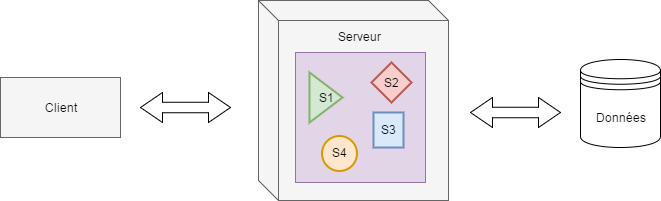
\includegraphics[scale=0.5]{images/travailNeuflizeOBC/architecture/troisTiers.png}
	\centering
	\caption{Architecture trois tiers monolithique}
	\label{troisTiers}
\end{figure}
	
	L'ensemble des services est contenu dans la même application et ces derniers sont donc exécutés dans un même processus. Ainsi, le moindre changement nécessite de rebuild et redéployer l'application entièrement. La scalabilité horizontale (par exemple un ajout de serveur) en est impactée. En effet, l'application entière doit être migrée si l'on souhaite changer de matériels afin d'améliorer les performances. Si un certain module est plus lent, il n'est pas possible de le déplacer indépendemment afin d'améliorer son exécution, il faut répliquer le monolithe entier tandis que du côté des microservices il est possible de répliquer un service en particulier et d'en redéployer un sans avoir à redéployer tout l'ensemble. De plus, dans les gros projets, la quantité de code a tendance à augmenter rapidement impliquant une hausse de la compléxité et rendant ainsi difficile l'ajout de nouvelles fonctionnalités. Le couplage entre ces dernières devient fort et les nombreux effets de bords résultant de chaque modifications rendent alors l'application moins fiable, limitant les perspectives d'évolution.

\begin{figure}[h!]
    \begin{minipage}{.5\textwidth}
    \raggedright
		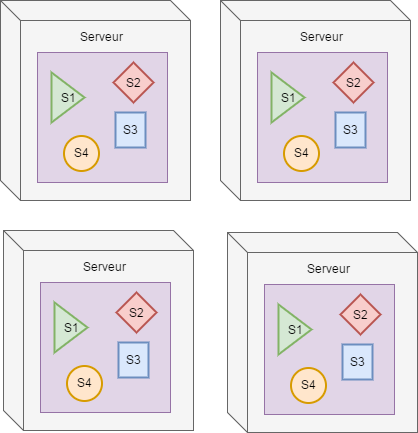
\includegraphics[scale=0.55]{images/travailNeuflizeOBC/architecture/monolithScale.png}
		\caption{Scalabilité horizontale d'une application monolithique \\}
		\label{monolithScale}
    \end{minipage}%
    \hspace{0.5cm}
    \begin{minipage}{.5\textwidth}
        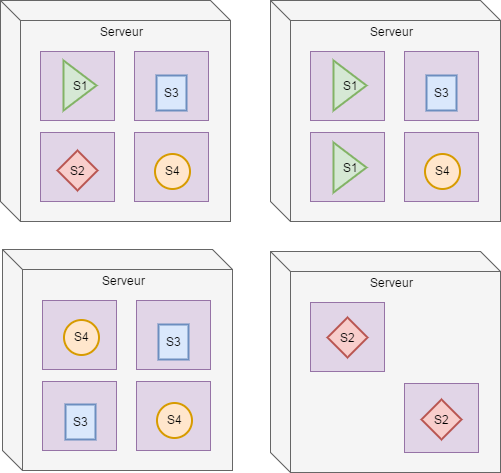
\includegraphics[scale=0.5]{images/travailNeuflizeOBC/architecture/microservicesScale.png}
		\caption{Scalabilité horizontale des microservices \\}
		\label{microservicesScale}
    \end{minipage}
\end{figure}

		Dans notre cas, l'objectif de la couche microservices , située dans le tiers 2, est de réaliser la composition des services métiers exposés par EFS dans le but d'exposer les données pour les applications ou les partenaires (comme PBI dont nous avons parlé dans la partie \ref{prezAppNeuflize}) qui viendront les consommer. Cette dernière est constituée des éléments présents sur la figure \ref{coucheMicroservices}. Les services EFS sont exposés via une surcouche API, située dans le tiers 2. \\

\begin{figure}[h!]
\raggedleft
	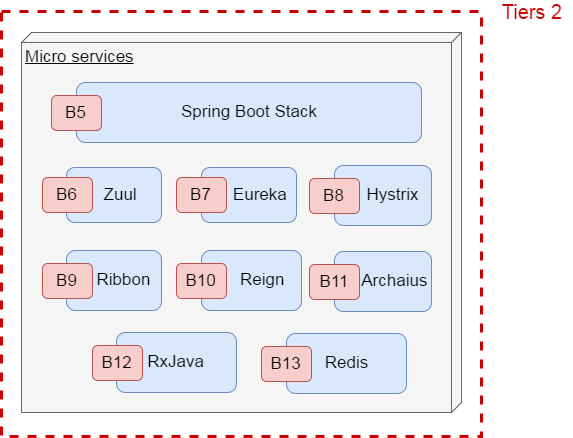
\includegraphics[scale=0.5]{images/travailNeuflizeOBC/architecture/coucheMicroservices.png}
	\centering
	\caption{Couche microservices}
	\label{coucheMicroservices}
\end{figure}
	
	\textit{Spring Boot Stack} est la brique applicative hébergeant les microservices. C’est dans cette dernière que la composition de services EFS est réalisée. Spring boot permet d'utiliser le framework java \textit{Spring} en simplifiant grandement la configuration, le déploiement ou encore la sécurité et en créant des applications cloud-ready.
	Cette brique prend aussi en charge l’implémentation des principaux patterns à savoir : \\
	
\begin{itemize}
	\item Circuit breaker : Capacité du système à être tolérant à la panne. En cas d’erreur successive lors de l’appel d’un sous-composant, le circuit d’appel est coupé « temporairement » en adoptant un comportement par défaut. L'implémentation qui a été choisie pour ce pattern est Hystrix de la stack \textit{Netflix OSS} \cite{bib_hystrix} permettant de contrôler la latence et les erreurs dues à des appels réseaux. L'idée essentielle est d'empêcher les erreurs en cascade dans un environnement distribué. Hystrix permet de \textit{fail-fast} mais de se rétablir rapidement créant ainsi une architecture tolérante aux erreurs capable de se remettre de manière autonome (on parle de self-heal). Ainsi, dès sa conception, le système prévoit les pannes.
	\item Feature toggle : Le principe est d’avoir une branche de développement et de déployer en production en continu. Ensuite, l’activation d’une « feature » est pilotée par le business. Cela permet aussi d’activer une fonctionnalité en fonction d’une population ou une stratégie particulière. \\
\end{itemize}

	Le serveur d'annuaire, essentielle à une architceture distribuée, permet la détection automatique des instances déployées. Les instances des applications sont accédées via leur nom (par exemple account-service) plutôt que par leurs adresses physiques/IPs. Les applications n'ont plus besoin de connaitre les adresses des instances. L'implémentation de l'annuaire de service est Eureka de la stack \textit{Netflix OSS} \cite{bib_eureka}. Les applications clientes peuvent s'enregistrer sur Eureka, via une annotation, qui fournira des metadatas telles que l'URL, le port ou encore le fil de vie (heathcheck) des instances. Eureka reçoit des messages dits "heartbeat" provenant de ces applications, si aucun message n'est reçu, en fonction d'un temps configurable, il supprimera l'instance. \\

	Ensuite, le point d'entrée unique de l'architecture microservices est sa gateway fournissant des services de routage dynamique, surveillance, résilience et sécurité. L'implémentation choisie est Zuul de la stack \textit{Netflix OSS} \cite{bib_zuul}. L'affichage d'une page web ou mobile peut nécessiter l'appel à une dizaine de microservices différents. Il n'est pas envisageable pour l'application cliente de connaitre l'ensemble des adresses physiques des microservices. Pour répondre à cette problématique, la gateway devient la seule adresse à connaitre pour les applications clientes. Zuul est aussi utilisé pour router les requêtes vers les services adéquats. Celui-ci retrouve les adresses des services automatiquement en interrogeant Eureka. Cependant, les services EFS et d'authentification (Axway gateway) sont paramétrés manuellement puisqu'ils ne sont pas enregistrés sur Eureka. La charge sera ensuite répartie grâce à un autre outils de Netflix, Ribbon, qui fourni des fonctionnalités de load-balancing permettant de distribuer la charge de travail. \\